\documentclass[11pt]{article}
\usepackage[textwidth=18.0cm, textheight=23.0cm, top=2.0cm]{geometry}
\usepackage{pst-all}
\usepackage{amssymb}
\usepackage{tikz}
\usepackage{underscore}\begin{document}
\pagestyle{empty}


ClassName: \underline{\textbf{Class_08.2bp-16}}
\par
BinSize: \underline{\textbf{100 × 100}}
\par
ReduceSize: \underline{\textbf{100 × 100}}
\par
TypeNum: \underline{\textbf{39}}
\par
Num: \underline{\textbf{40}}
\par
OutS: \underline{\textbf{110000}}
\par
InS: \underline{\textbf{88625}}
\par
Rate: \underline{\textbf{0.806}}
\par
UB: \underline{\textbf{11}}
\par
LB0: \underline{\textbf{11}}
\par
LB: \underline{\textbf{11}}
\par
LBWithCut: \underline{\textbf{11}}
\par
NodeCut: \underline{\textbf{0}}
\par
ExtendedNodeCnt: \underline{\textbf{1}}
\par
GenNodeCnt: \underline{\textbf{1}}
\par
PrimalNode: \underline{\textbf{0}}
\par
ColumnCount: \underline{\textbf{11}}
\par
TotalCutCount: \underline{\textbf{0}}
\par
RootCutCount: \underline{\textbf{0}}
\par
LPSolverCnt: \underline{\textbf{1}}
\par
PricingSolverCnt: \underline{\textbf{0}}
\par
BranchAndBoundNum: \underline{\textbf{1}}
\par
isOpt: \underline{\textbf{true}}
\par
TimeOnInitSolution: \underline{\textbf{600.000 s}}
\par
TimeOnPrimal: \underline{\textbf{0.000 s}}
\par
TimeOnPricing: \underline{\textbf{0.000 s}}
\par
TimeOnRmp: \underline{\textbf{0.047 s}}
\par
TotalTime: \underline{\textbf{600.281 s}}
\par
\newpage


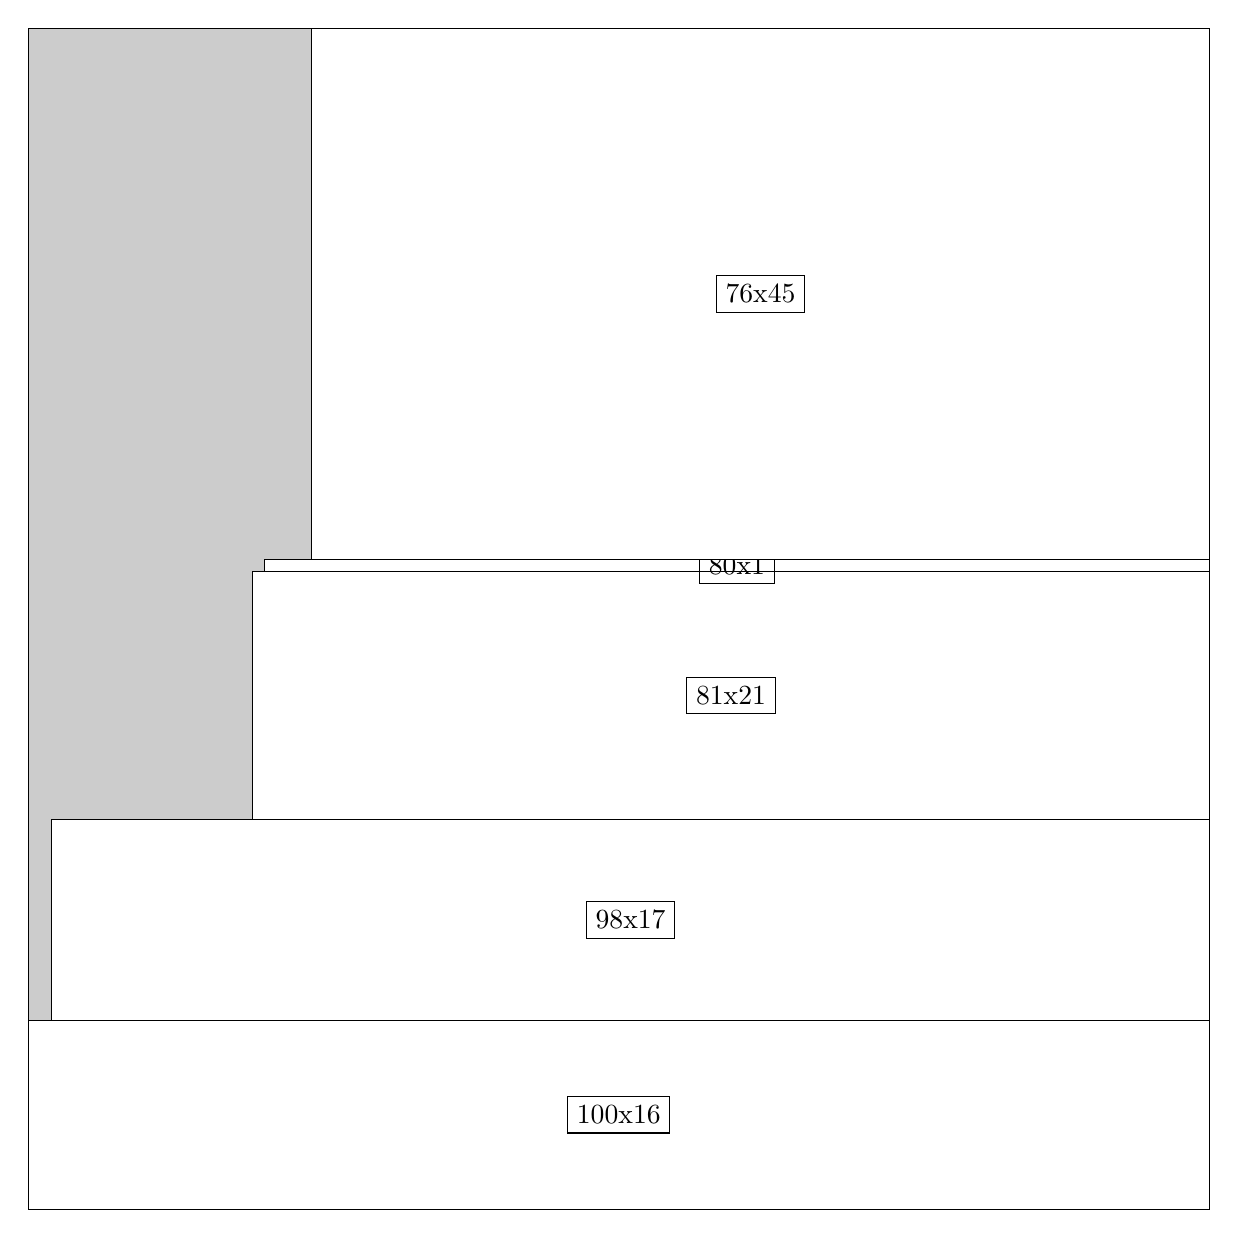
\begin{tikzpicture}[shorten >=1pt,scale=1.0,every node/.style={scale=1.0},->]
\tikzstyle{vertex}=[circle,fill=black!25,minimum size=14pt,inner sep=0pt]
\filldraw[fill=gray!40!white, draw=black] (0,0) rectangle (15.0,15.0);
\foreach \name/\x/\y/\w/\h in {100x16/0.0/0.0/15.0/2.4,98x17/0.3/2.4/14.7/2.55,81x21/2.85/4.95/12.15/3.15,80x1/3.0/8.1/12.0/0.15,76x45/3.5999999999999996/8.25/11.4/6.75}
\filldraw[fill=white!40!white, draw=black] (\x,\y) rectangle node[draw] (\name) {\name} ++(\w,\h);
\end{tikzpicture}


w =100 , h =16 , x =0 , y =0 , v =1600
\par
w =98 , h =17 , x =2 , y =16 , v =1666
\par
w =81 , h =21 , x =19 , y =33 , v =1701
\par
w =80 , h =1 , x =20 , y =54 , v =80
\par
w =76 , h =45 , x =24 , y =55 , v =3420
\par
\newpage


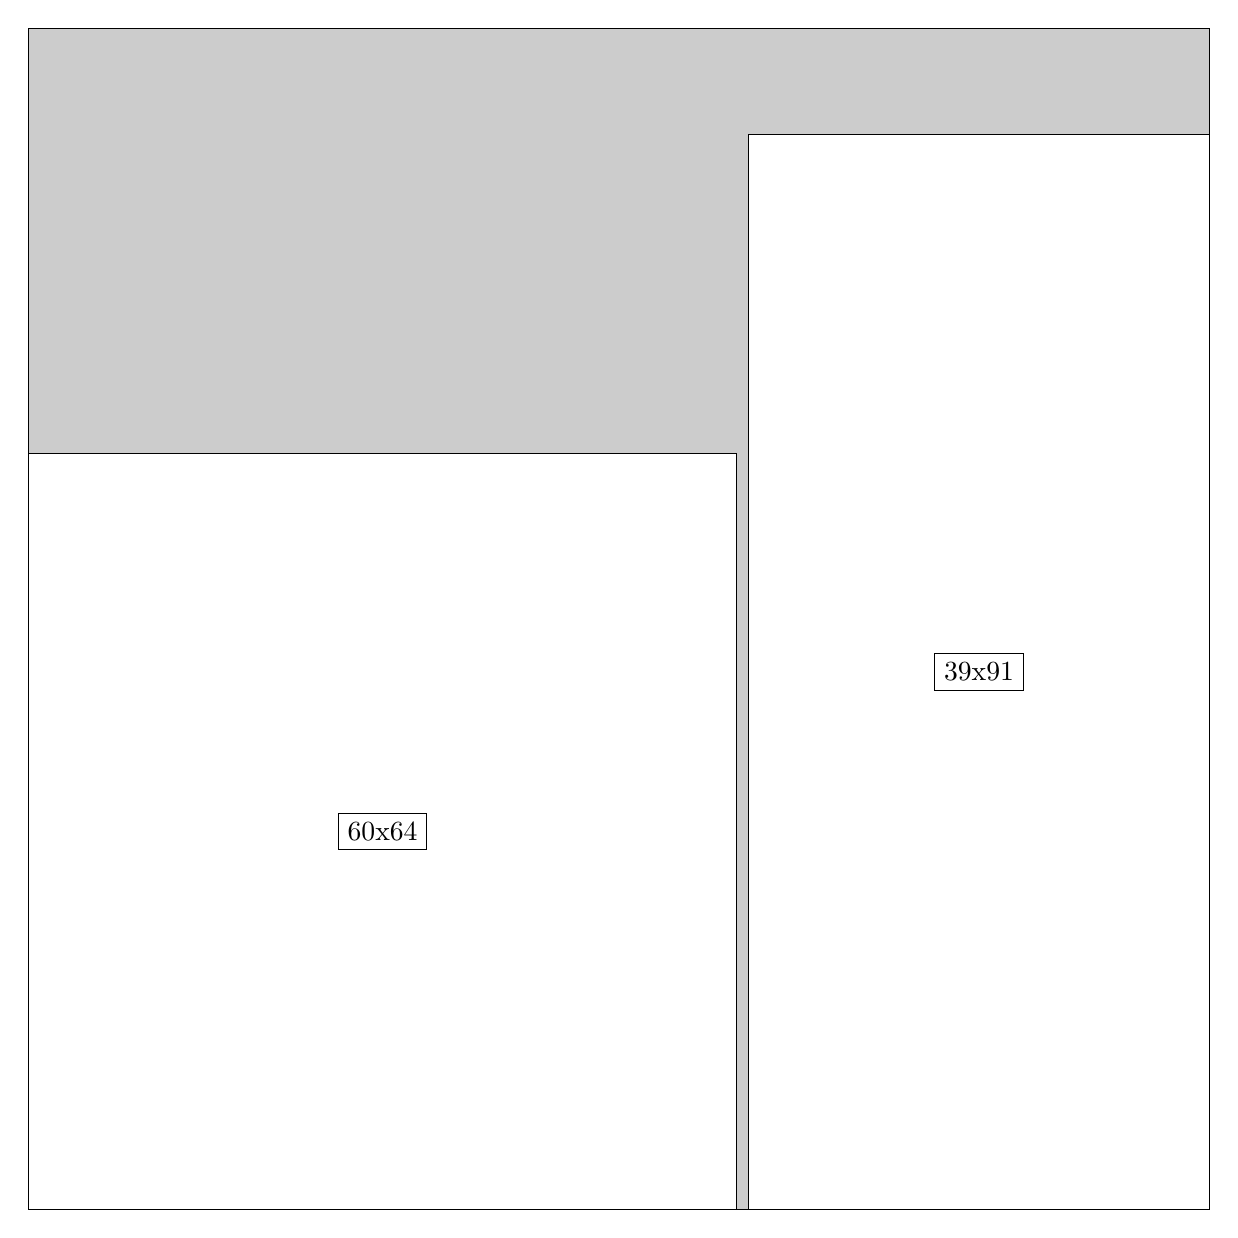
\begin{tikzpicture}[shorten >=1pt,scale=1.0,every node/.style={scale=1.0},->]
\tikzstyle{vertex}=[circle,fill=black!25,minimum size=14pt,inner sep=0pt]
\filldraw[fill=gray!40!white, draw=black] (0,0) rectangle (15.0,15.0);
\foreach \name/\x/\y/\w/\h in {39x91/9.15/0.0/5.85/13.65,60x64/0.0/0.0/9.0/9.6}
\filldraw[fill=white!40!white, draw=black] (\x,\y) rectangle node[draw] (\name) {\name} ++(\w,\h);
\end{tikzpicture}


w =39 , h =91 , x =61 , y =0 , v =3549
\par
w =60 , h =64 , x =0 , y =0 , v =3840
\par
\newpage


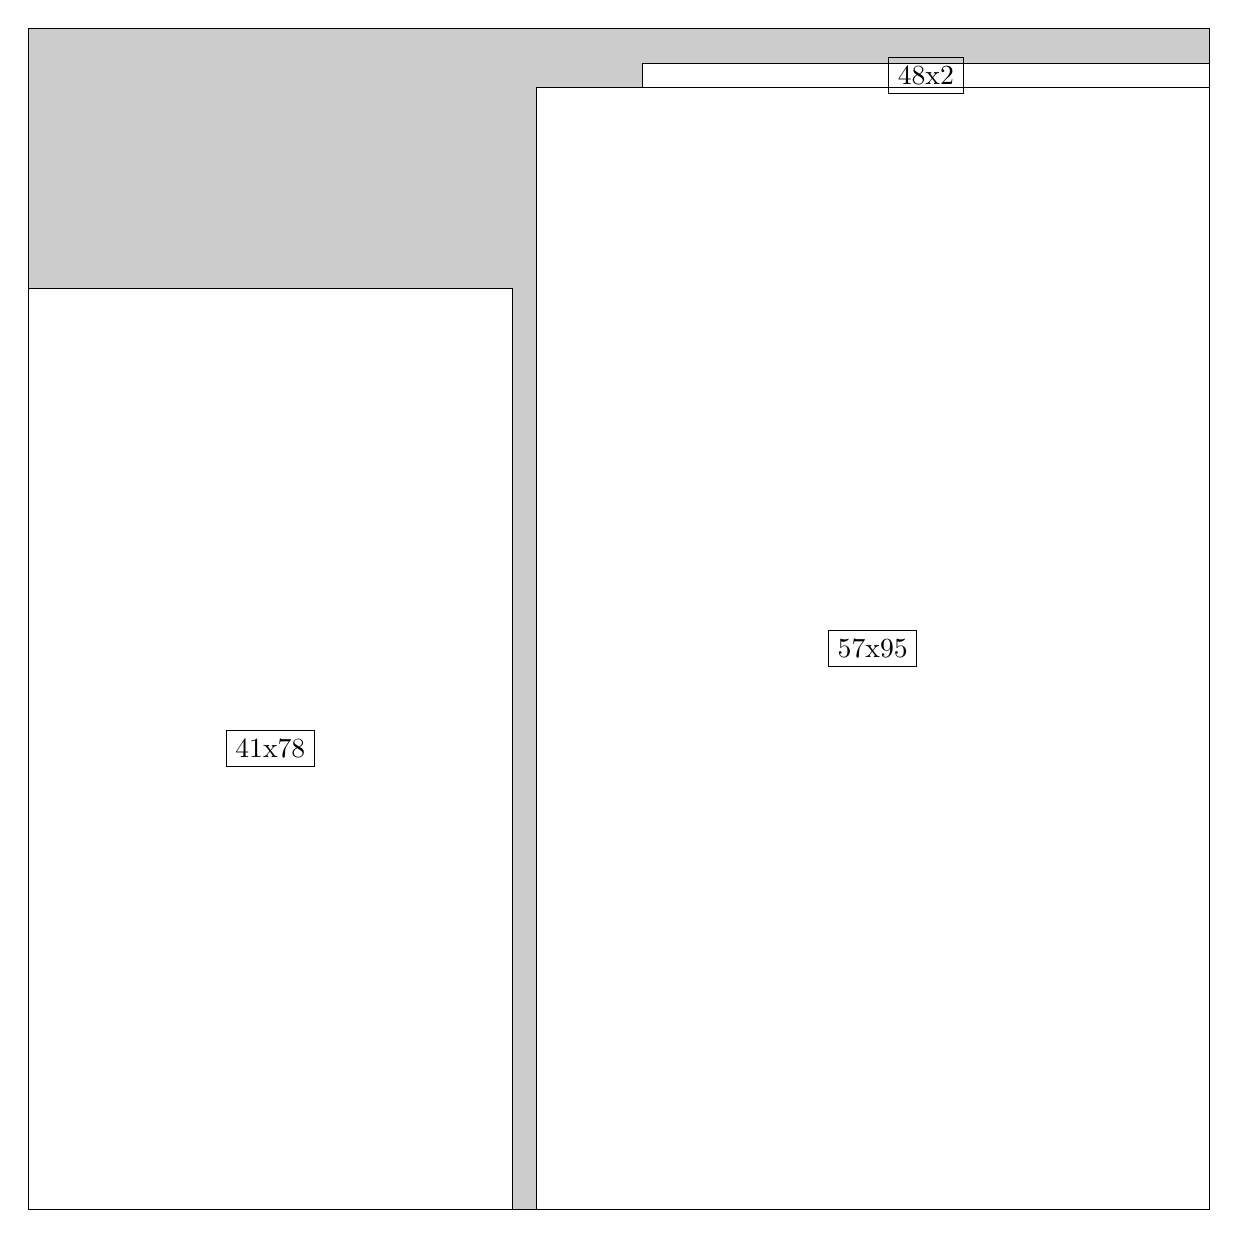
\begin{tikzpicture}[shorten >=1pt,scale=1.0,every node/.style={scale=1.0},->]
\tikzstyle{vertex}=[circle,fill=black!25,minimum size=14pt,inner sep=0pt]
\filldraw[fill=gray!40!white, draw=black] (0,0) rectangle (15.0,15.0);
\foreach \name/\x/\y/\w/\h in {57x95/6.45/0.0/8.549999999999999/14.25,48x2/7.8/14.25/7.199999999999999/0.3,41x78/0.0/0.0/6.1499999999999995/11.7}
\filldraw[fill=white!40!white, draw=black] (\x,\y) rectangle node[draw] (\name) {\name} ++(\w,\h);
\end{tikzpicture}


w =57 , h =95 , x =43 , y =0 , v =5415
\par
w =48 , h =2 , x =52 , y =95 , v =96
\par
w =41 , h =78 , x =0 , y =0 , v =3198
\par
\newpage


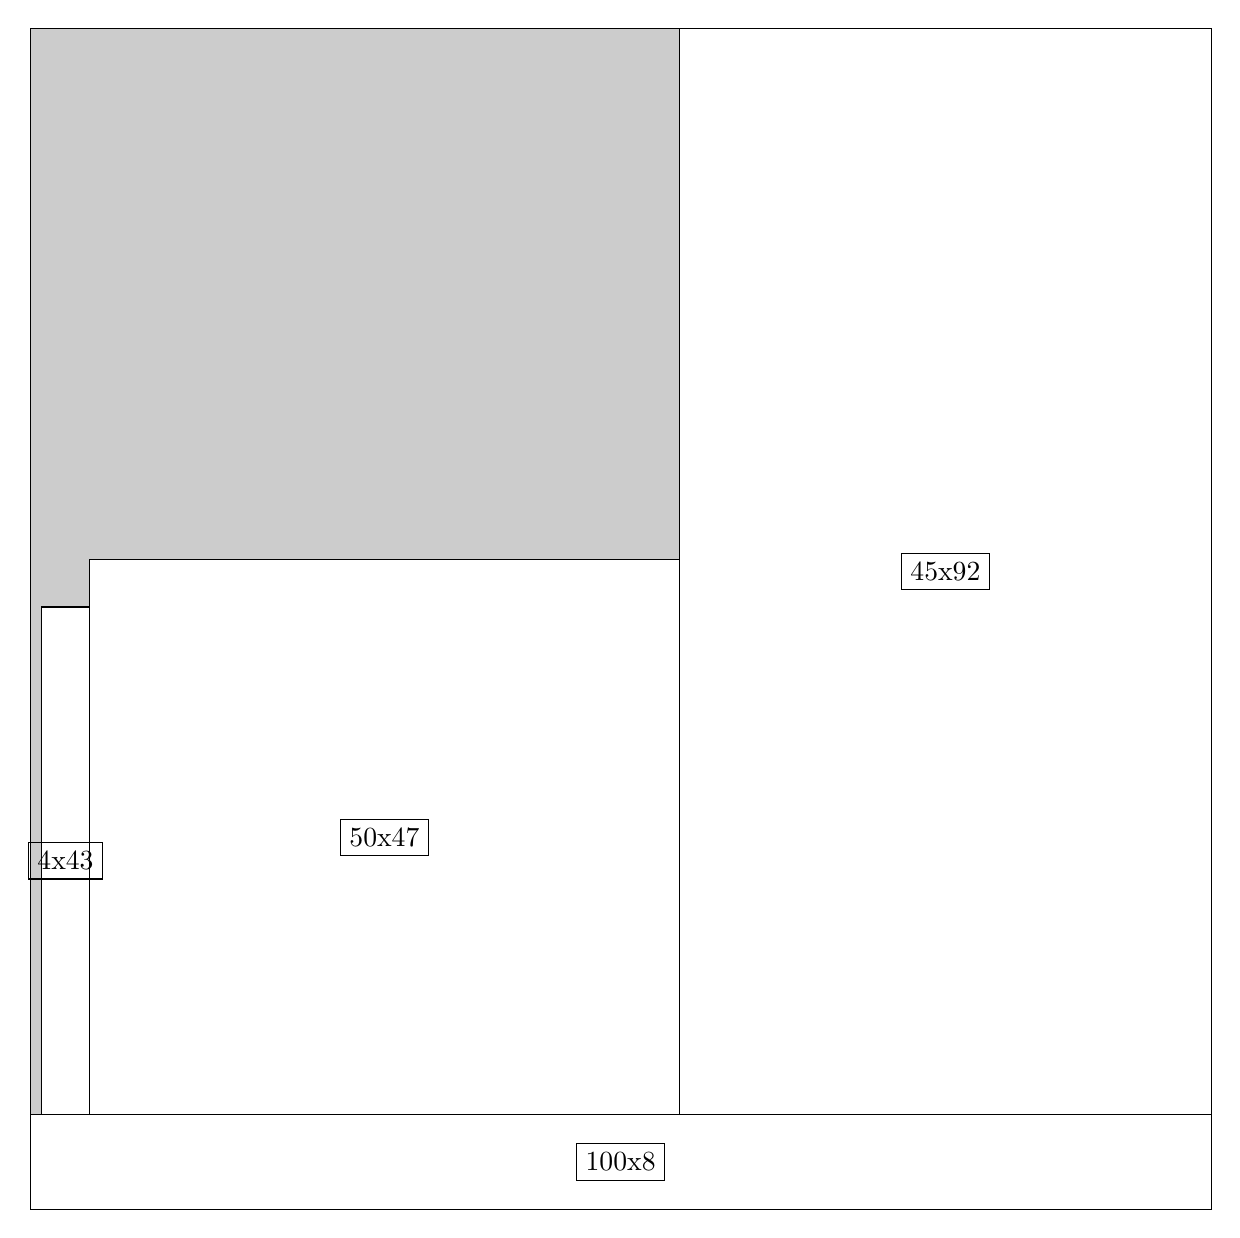
\begin{tikzpicture}[shorten >=1pt,scale=1.0,every node/.style={scale=1.0},->]
\tikzstyle{vertex}=[circle,fill=black!25,minimum size=14pt,inner sep=0pt]
\filldraw[fill=gray!40!white, draw=black] (0,0) rectangle (15.0,15.0);
\foreach \name/\x/\y/\w/\h in {100x8/0.0/0.0/15.0/1.2,45x92/8.25/1.2/6.75/13.799999999999999,50x47/0.75/1.2/7.5/7.05,4x43/0.15/1.2/0.6/6.45}
\filldraw[fill=white!40!white, draw=black] (\x,\y) rectangle node[draw] (\name) {\name} ++(\w,\h);
\end{tikzpicture}


w =100 , h =8 , x =0 , y =0 , v =800
\par
w =45 , h =92 , x =55 , y =8 , v =4140
\par
w =50 , h =47 , x =5 , y =8 , v =2350
\par
w =4 , h =43 , x =1 , y =8 , v =172
\par
\newpage


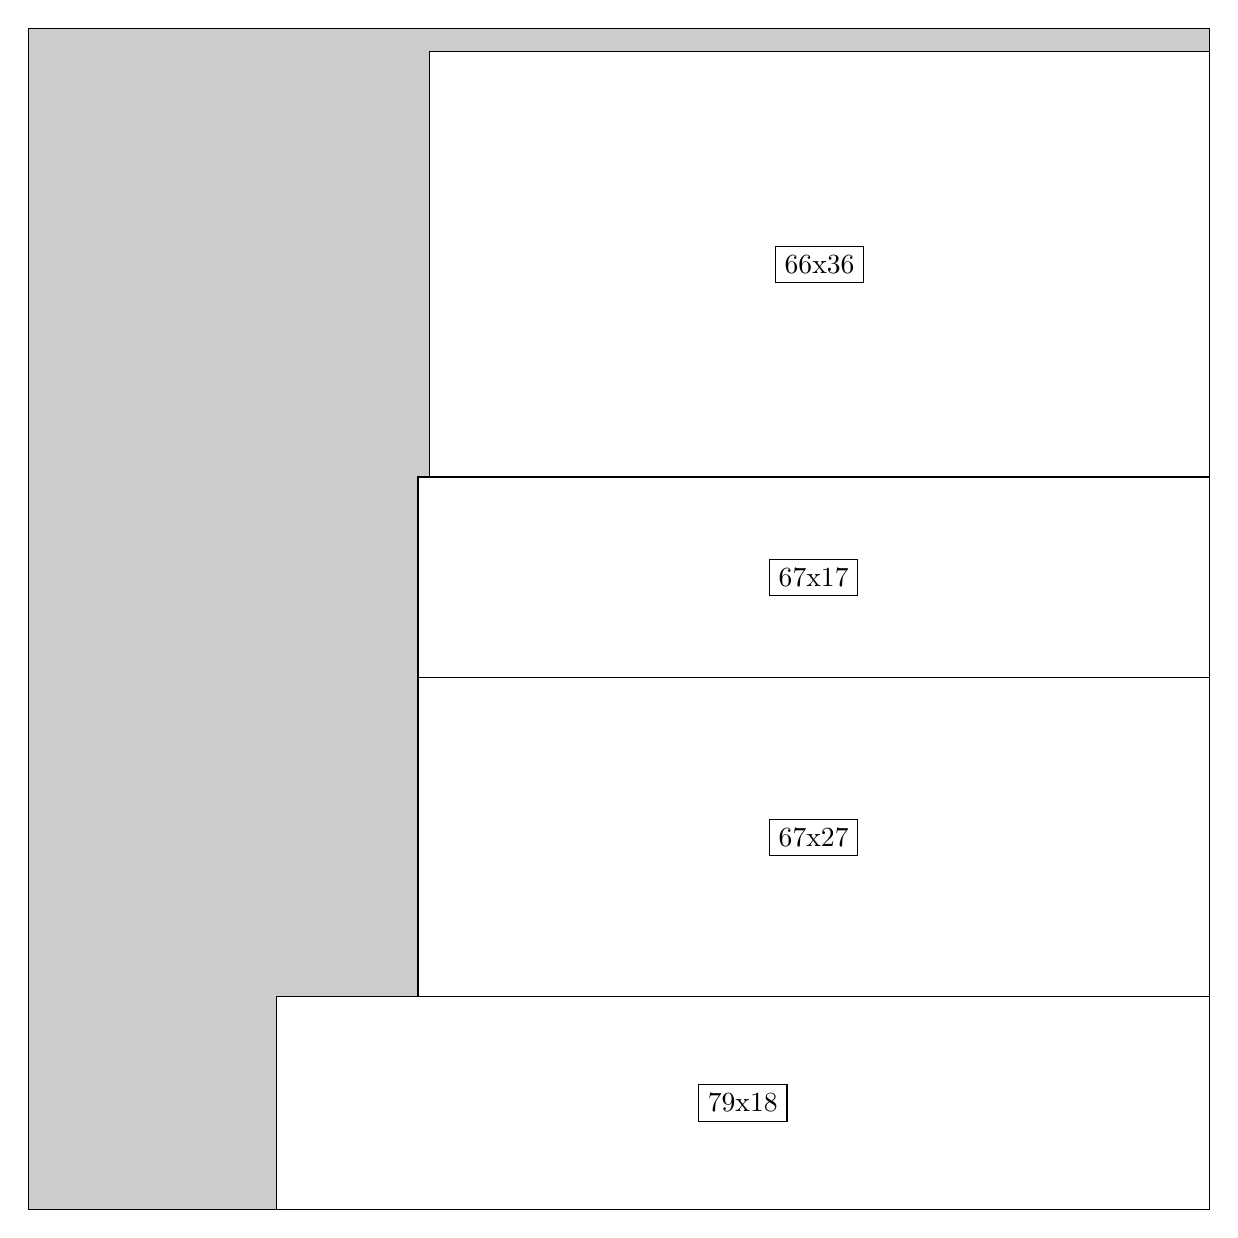
\begin{tikzpicture}[shorten >=1pt,scale=1.0,every node/.style={scale=1.0},->]
\tikzstyle{vertex}=[circle,fill=black!25,minimum size=14pt,inner sep=0pt]
\filldraw[fill=gray!40!white, draw=black] (0,0) rectangle (15.0,15.0);
\foreach \name/\x/\y/\w/\h in {79x18/3.15/0.0/11.85/2.6999999999999997,67x27/4.95/2.6999999999999997/10.049999999999999/4.05,67x17/4.95/6.75/10.049999999999999/2.55,66x36/5.1/9.299999999999999/9.9/5.3999999999999995}
\filldraw[fill=white!40!white, draw=black] (\x,\y) rectangle node[draw] (\name) {\name} ++(\w,\h);
\end{tikzpicture}


w =79 , h =18 , x =21 , y =0 , v =1422
\par
w =67 , h =27 , x =33 , y =18 , v =1809
\par
w =67 , h =17 , x =33 , y =45 , v =1139
\par
w =66 , h =36 , x =34 , y =62 , v =2376
\par
\newpage


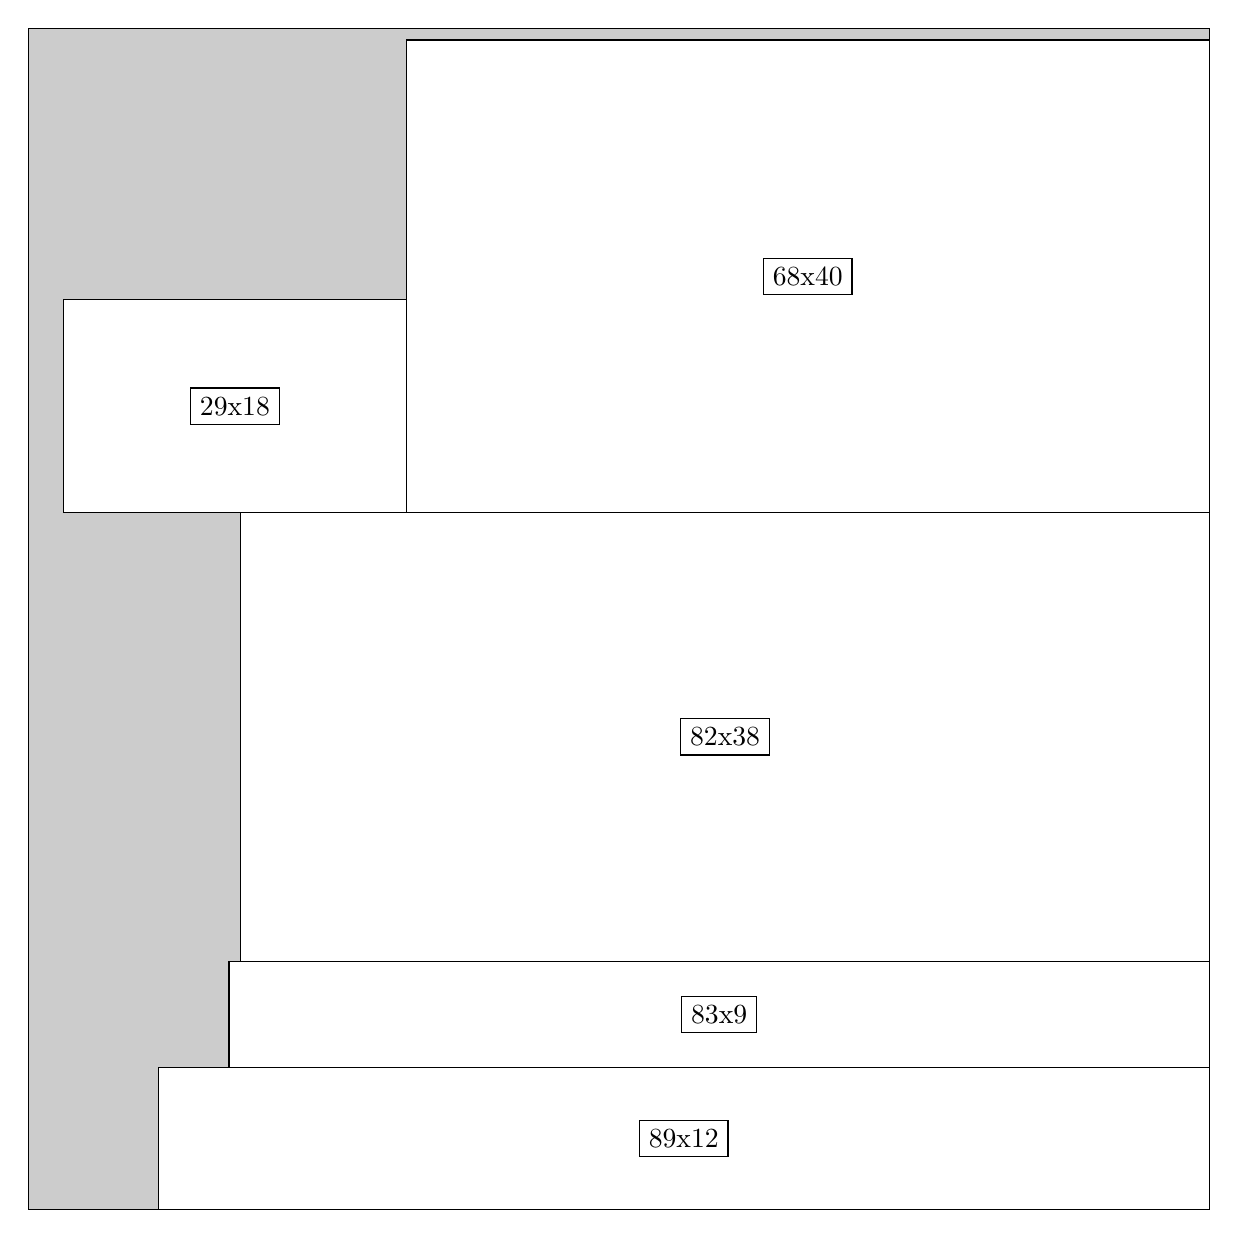
\begin{tikzpicture}[shorten >=1pt,scale=1.0,every node/.style={scale=1.0},->]
\tikzstyle{vertex}=[circle,fill=black!25,minimum size=14pt,inner sep=0pt]
\filldraw[fill=gray!40!white, draw=black] (0,0) rectangle (15.0,15.0);
\foreach \name/\x/\y/\w/\h in {89x12/1.65/0.0/13.35/1.7999999999999998,83x9/2.55/1.7999999999999998/12.45/1.3499999999999999,82x38/2.6999999999999997/3.15/12.299999999999999/5.7,68x40/4.8/8.85/10.2/6.0,29x18/0.44999999999999996/8.85/4.35/2.6999999999999997}
\filldraw[fill=white!40!white, draw=black] (\x,\y) rectangle node[draw] (\name) {\name} ++(\w,\h);
\end{tikzpicture}


w =89 , h =12 , x =11 , y =0 , v =1068
\par
w =83 , h =9 , x =17 , y =12 , v =747
\par
w =82 , h =38 , x =18 , y =21 , v =3116
\par
w =68 , h =40 , x =32 , y =59 , v =2720
\par
w =29 , h =18 , x =3 , y =59 , v =522
\par
\newpage


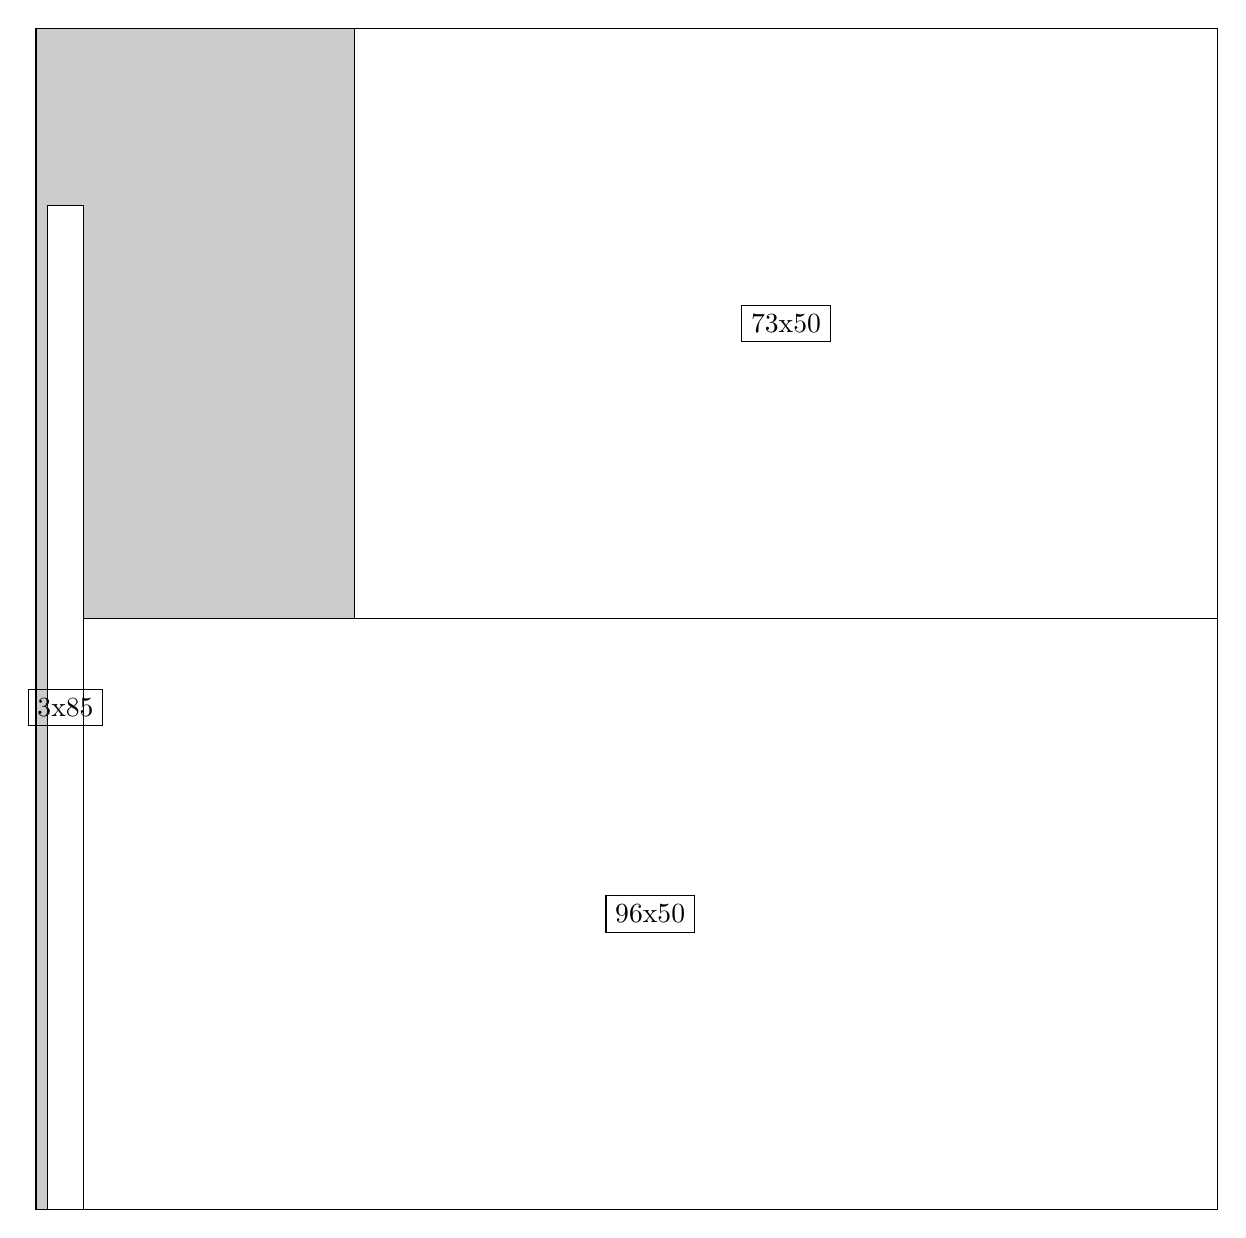
\begin{tikzpicture}[shorten >=1pt,scale=1.0,every node/.style={scale=1.0},->]
\tikzstyle{vertex}=[circle,fill=black!25,minimum size=14pt,inner sep=0pt]
\filldraw[fill=gray!40!white, draw=black] (0,0) rectangle (15.0,15.0);
\foreach \name/\x/\y/\w/\h in {96x50/0.6/0.0/14.399999999999999/7.5,73x50/4.05/7.5/10.95/7.5,3x85/0.15/0.0/0.44999999999999996/12.75}
\filldraw[fill=white!40!white, draw=black] (\x,\y) rectangle node[draw] (\name) {\name} ++(\w,\h);
\end{tikzpicture}


w =96 , h =50 , x =4 , y =0 , v =4800
\par
w =73 , h =50 , x =27 , y =50 , v =3650
\par
w =3 , h =85 , x =1 , y =0 , v =255
\par
\newpage


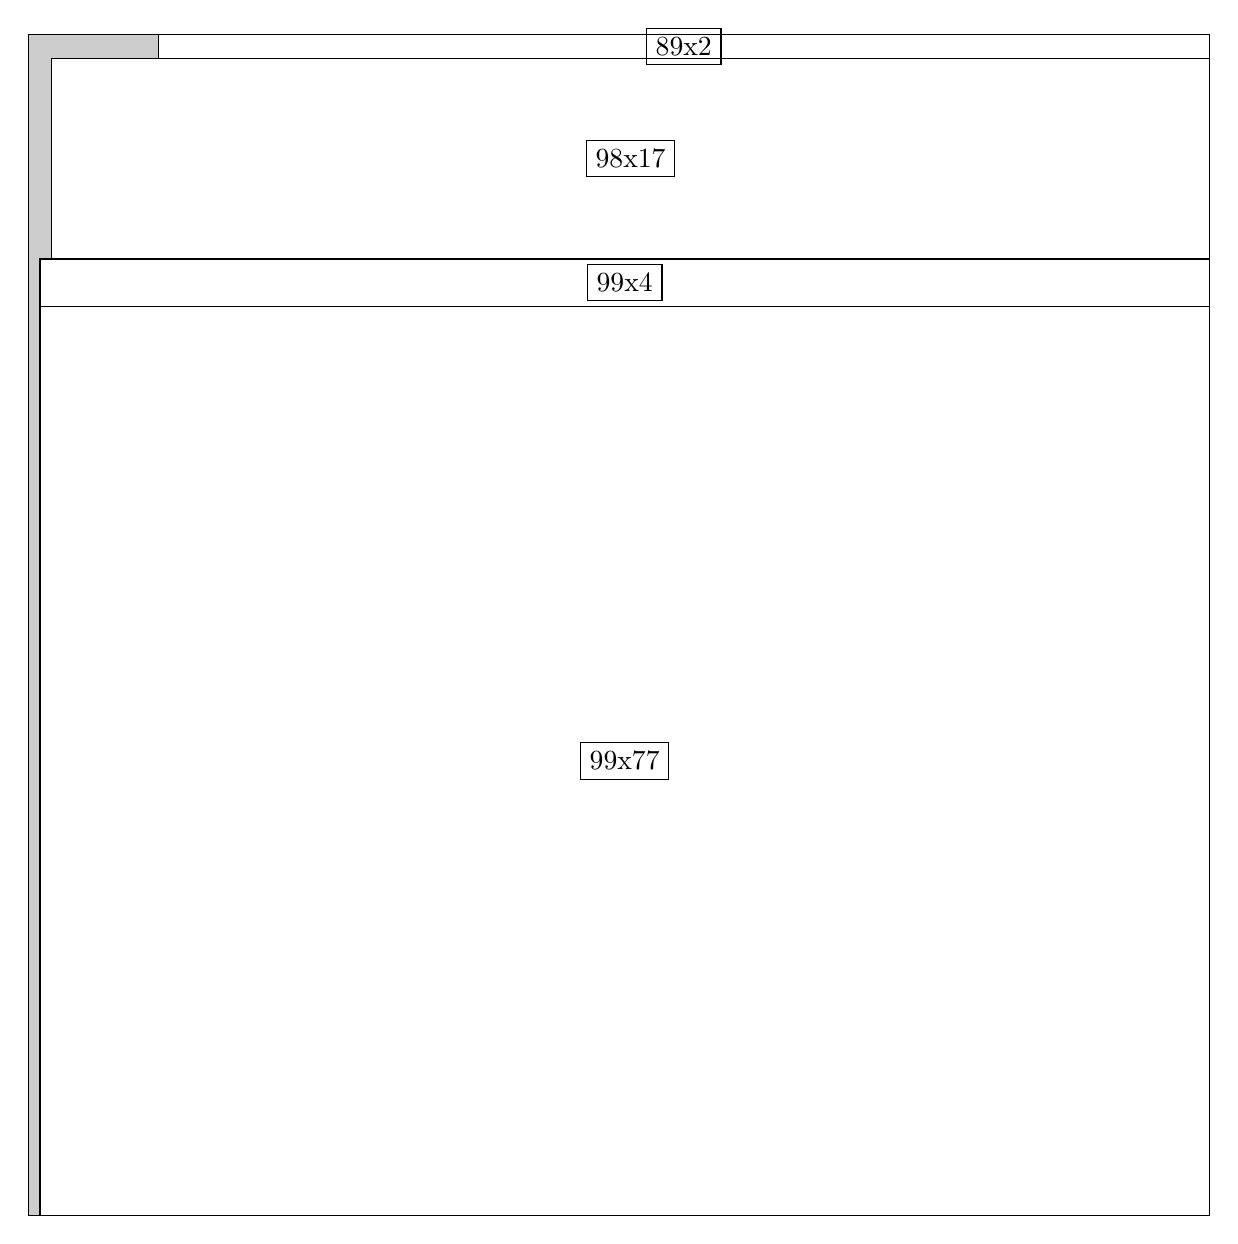
\begin{tikzpicture}[shorten >=1pt,scale=1.0,every node/.style={scale=1.0},->]
\tikzstyle{vertex}=[circle,fill=black!25,minimum size=14pt,inner sep=0pt]
\filldraw[fill=gray!40!white, draw=black] (0,0) rectangle (15.0,15.0);
\foreach \name/\x/\y/\w/\h in {99x77/0.15/0.0/14.85/11.549999999999999,99x4/0.15/11.549999999999999/14.85/0.6,98x17/0.3/12.15/14.7/2.55,89x2/1.65/14.7/13.35/0.3}
\filldraw[fill=white!40!white, draw=black] (\x,\y) rectangle node[draw] (\name) {\name} ++(\w,\h);
\end{tikzpicture}


w =99 , h =77 , x =1 , y =0 , v =7623
\par
w =99 , h =4 , x =1 , y =77 , v =396
\par
w =98 , h =17 , x =2 , y =81 , v =1666
\par
w =89 , h =2 , x =11 , y =98 , v =178
\par
\newpage


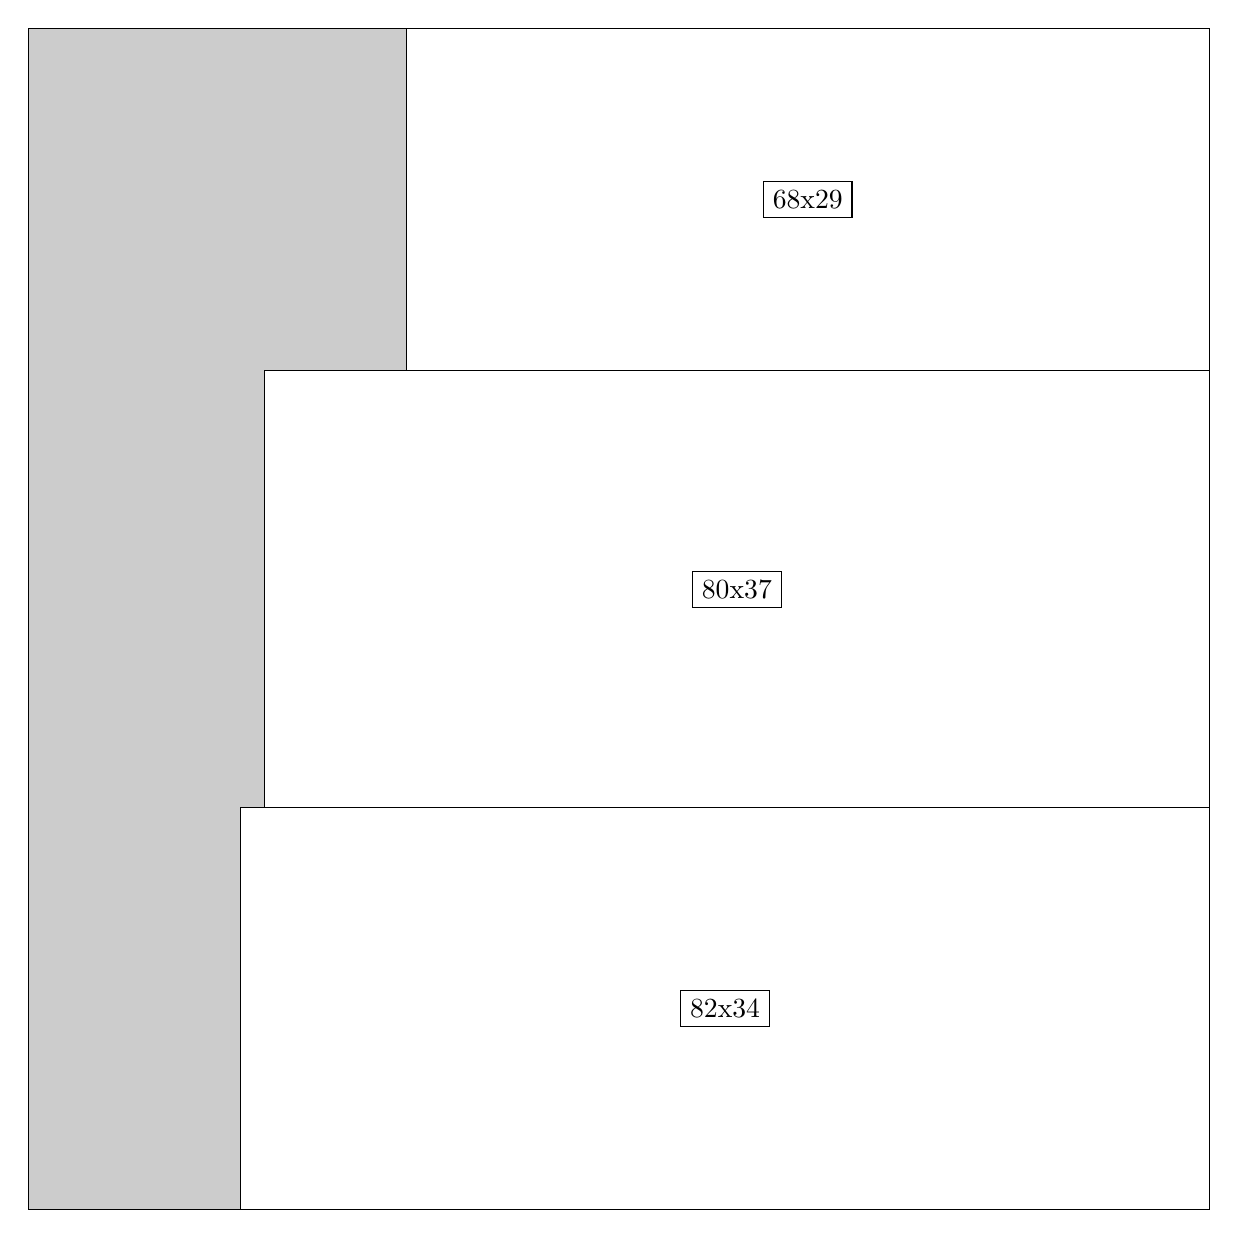
\begin{tikzpicture}[shorten >=1pt,scale=1.0,every node/.style={scale=1.0},->]
\tikzstyle{vertex}=[circle,fill=black!25,minimum size=14pt,inner sep=0pt]
\filldraw[fill=gray!40!white, draw=black] (0,0) rectangle (15.0,15.0);
\foreach \name/\x/\y/\w/\h in {82x34/2.6999999999999997/0.0/12.299999999999999/5.1,80x37/3.0/5.1/12.0/5.55,68x29/4.8/10.65/10.2/4.35}
\filldraw[fill=white!40!white, draw=black] (\x,\y) rectangle node[draw] (\name) {\name} ++(\w,\h);
\end{tikzpicture}


w =82 , h =34 , x =18 , y =0 , v =2788
\par
w =80 , h =37 , x =20 , y =34 , v =2960
\par
w =68 , h =29 , x =32 , y =71 , v =1972
\par
\newpage


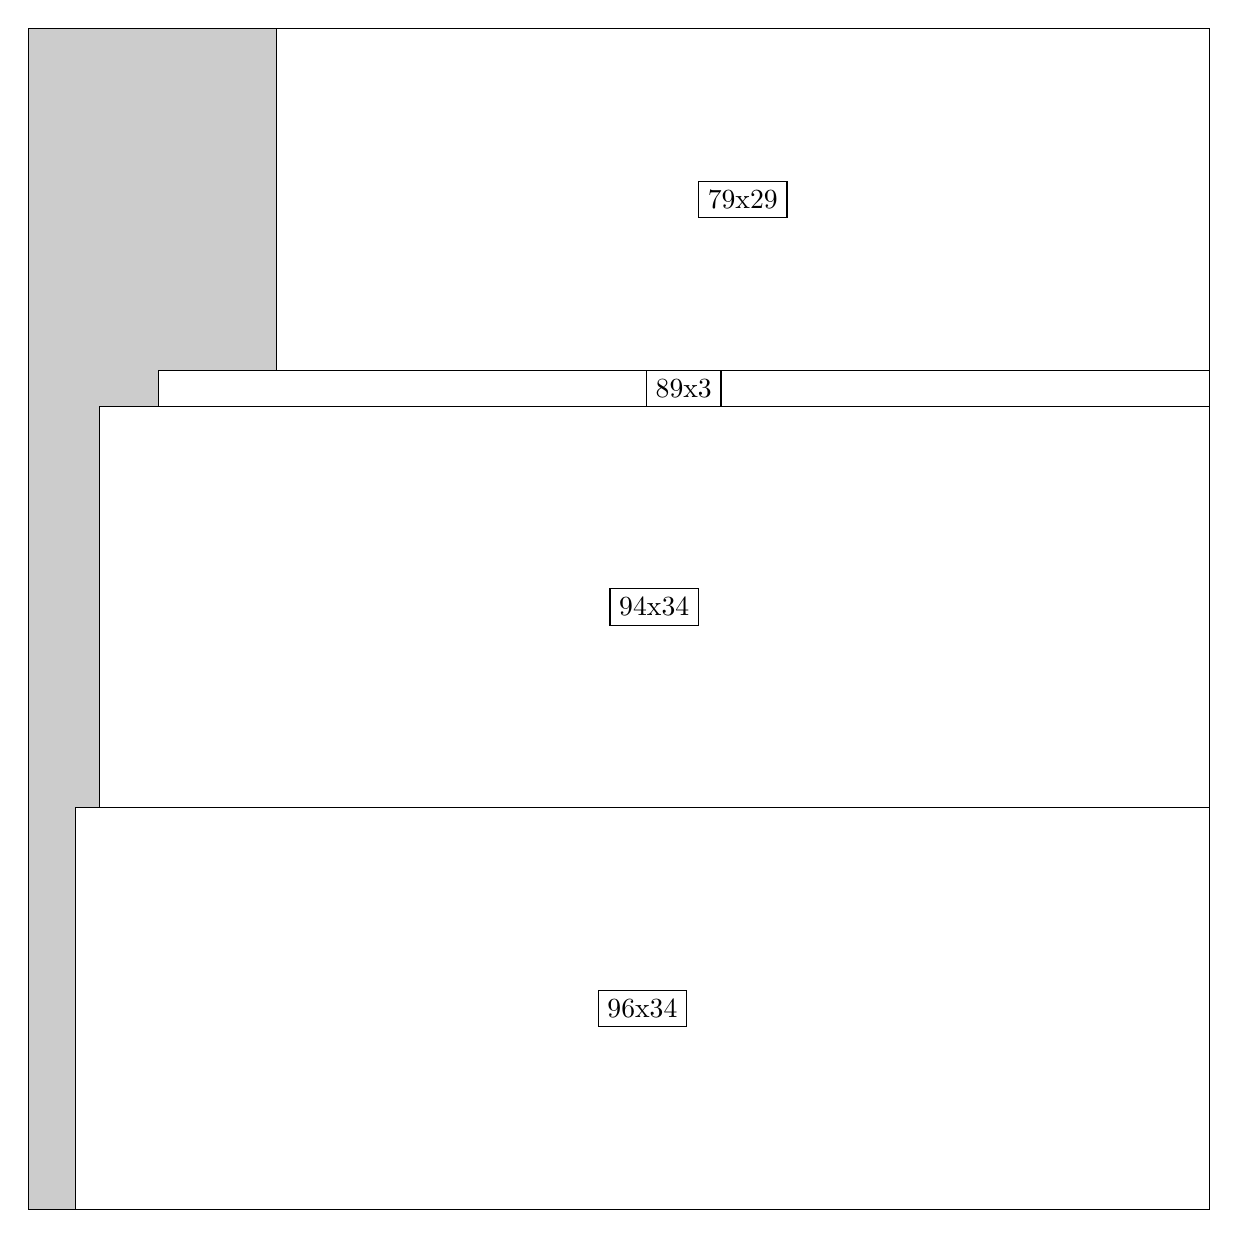
\begin{tikzpicture}[shorten >=1pt,scale=1.0,every node/.style={scale=1.0},->]
\tikzstyle{vertex}=[circle,fill=black!25,minimum size=14pt,inner sep=0pt]
\filldraw[fill=gray!40!white, draw=black] (0,0) rectangle (15.0,15.0);
\foreach \name/\x/\y/\w/\h in {96x34/0.6/0.0/14.399999999999999/5.1,94x34/0.8999999999999999/5.1/14.1/5.1,89x3/1.65/10.2/13.35/0.44999999999999996,79x29/3.15/10.65/11.85/4.35}
\filldraw[fill=white!40!white, draw=black] (\x,\y) rectangle node[draw] (\name) {\name} ++(\w,\h);
\end{tikzpicture}


w =96 , h =34 , x =4 , y =0 , v =3264
\par
w =94 , h =34 , x =6 , y =34 , v =3196
\par
w =89 , h =3 , x =11 , y =68 , v =267
\par
w =79 , h =29 , x =21 , y =71 , v =2291
\par
\newpage


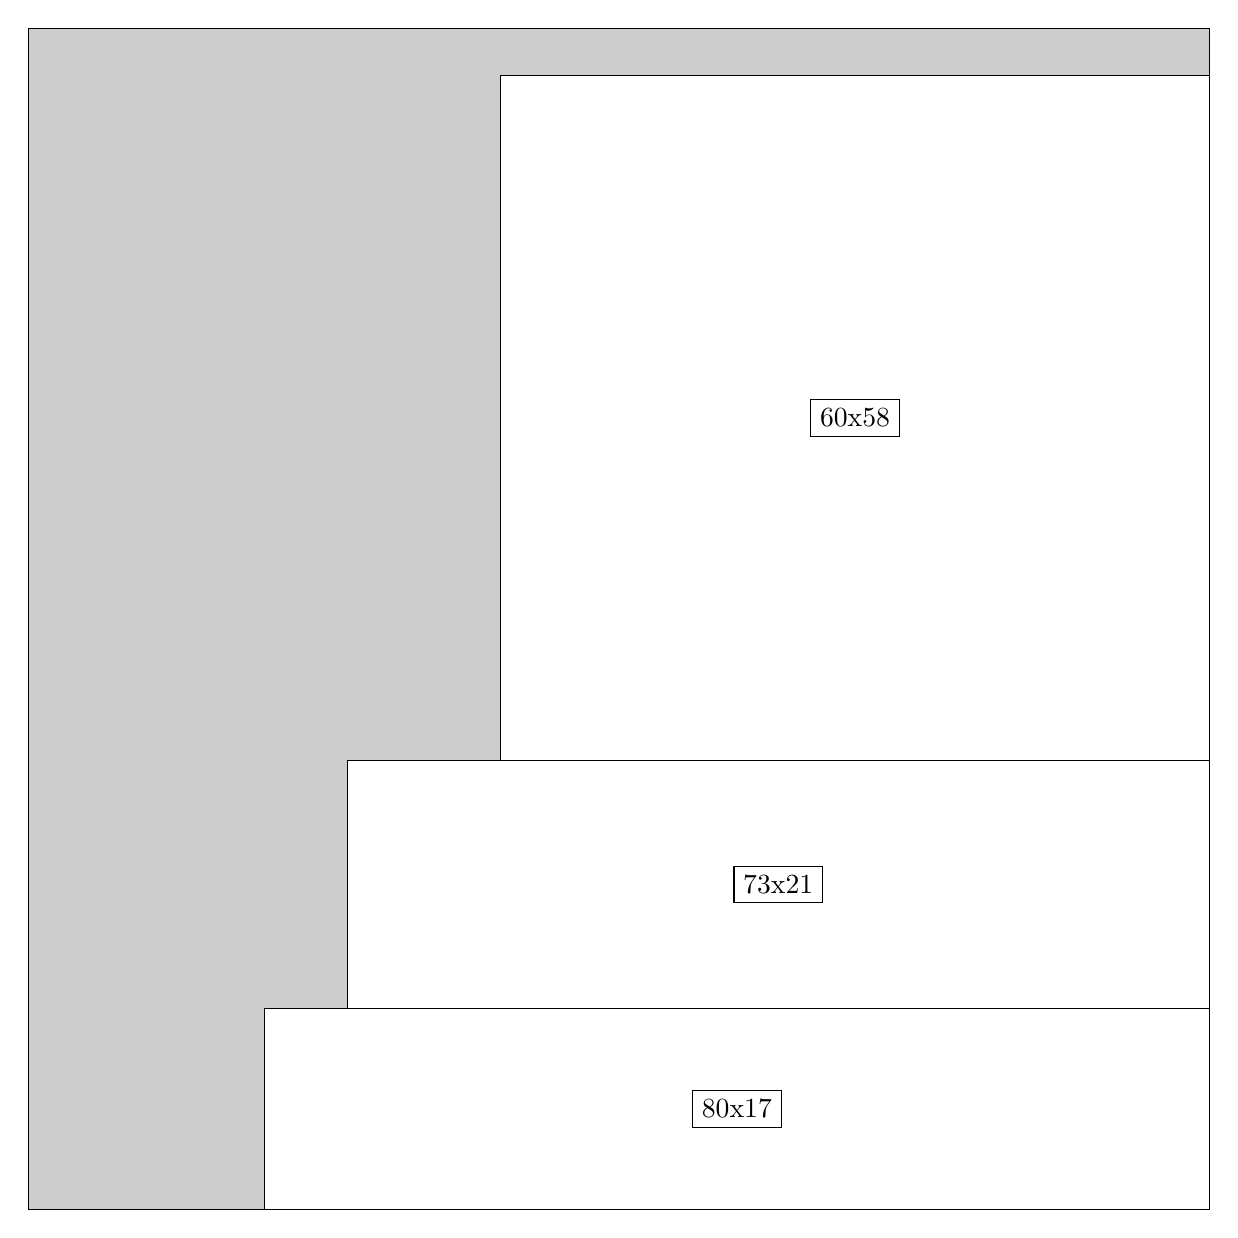
\begin{tikzpicture}[shorten >=1pt,scale=1.0,every node/.style={scale=1.0},->]
\tikzstyle{vertex}=[circle,fill=black!25,minimum size=14pt,inner sep=0pt]
\filldraw[fill=gray!40!white, draw=black] (0,0) rectangle (15.0,15.0);
\foreach \name/\x/\y/\w/\h in {80x17/3.0/0.0/12.0/2.55,73x21/4.05/2.55/10.95/3.15,60x58/6.0/5.7/9.0/8.7}
\filldraw[fill=white!40!white, draw=black] (\x,\y) rectangle node[draw] (\name) {\name} ++(\w,\h);
\end{tikzpicture}


w =80 , h =17 , x =20 , y =0 , v =1360
\par
w =73 , h =21 , x =27 , y =17 , v =1533
\par
w =60 , h =58 , x =40 , y =38 , v =3480
\par
\newpage


\end{document}